%!TEX root = ./../thesis.tex

\chapter{Framework}
\label{c:state_centric}
Most state-of-the-art frameworks for distributed machine learning like Petuum \cite{Xing2015} and Parameter Server \cite{Li2014} are based on the parameter server concept introduced in the previous section.
This framework essentially provides a low level API\footnote{Application programming interface} for publishing and retrieving values similar to a distributed key-value store, where the key $i$ is for example the index of a weight vector $w$ stored on the server and the value is the weight $w_i$.
Implementing an algorithm that relies on a parameter server requires incorporating publishing and retrieval of parameters deeply into the algorithm definition.
This contrasts the general work flow of developing and testing an algorithm locally on a single machine and then transition to a distributed environment such as a cluster.
Also current frameworks provide only a minor abstraction, leaving the developer with the task of distributing state, scheduling distributed computation, consistency management and managing cluster resources.
A developer should be able to focus on the main goal of distributed machine learning, namely an efficient parallel execution.
This section introduces the general architecture of the framework and its main parts based on the example of iterative-convergent algorithms, though its application is not limited to this particular family.

As depicted in Figure \ref{fig:framework_architecture} the framework consists of three major parts, designed to support the developer with the development and execution of distributed machine learning algorithms.
First, it provides a collection of primitives that can used to describe the algorithm with the help of a state centric programming model.
The SCPM\footnote{State-centric Programming Model} treats state as a first class citizen which can be distributed according to a given partitioning and altered by local and remote transformation in parallel.
Depending on how a state is distributed and the type of transformation applied to it, the consistency management coordinates the distributed execution of all algorithm steps in a way that ensures the correctness of the result.
In the context of machine learning, a correct result can be obtained in different ways as discussed in Section \ref{ss:consistency}.
Therefore additional primitives are offered by the framework to provide the consistency management with further instructions on how to ensure a consistent distributed execution given a particular state and transformation.
\begin{figure}[ht]
\centering
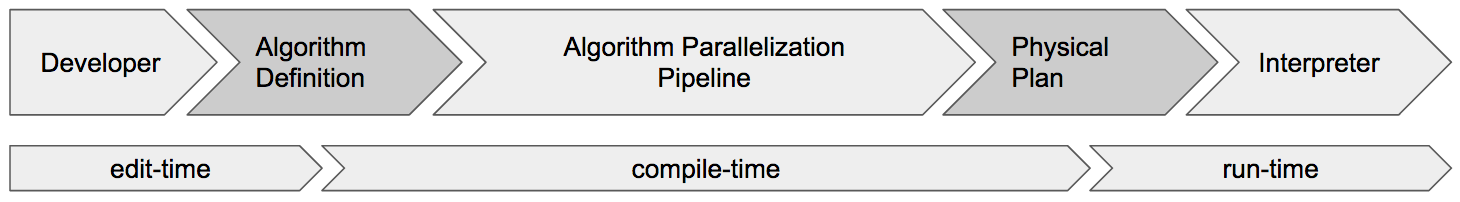
\includegraphics[width=0.9\textwidth]{img/framework_architecture.png}
\caption{Framework Architecture}
\label{fig:framework_architecture}
\end{figure}
Secondly, the framework provides an algorithm parallelization pipeline, which takes the algorithm definition as an input an compiles a physical plan by applying a sequence of enrichment steps to it.
These enrichment steps, as discussed in Section \ref{s:algo_parallel_pipeline}, take properties of the algorithm and cluster infrastructure into account to find the optimal execution strategy.
The physical plan contains a detailed description of how to execute the algorithm in a distributed manner on a specific group of machines within the cluster.
As the third and final part of the framework, the interpreter is responsible for translating the physical plan into a sequence of control instructions that are used to control the distributed execution of the algorithm among the participating machines, as can be seen in Figure \ref{fig:framework_driver}.
\begin{figure}[ht]
\centering
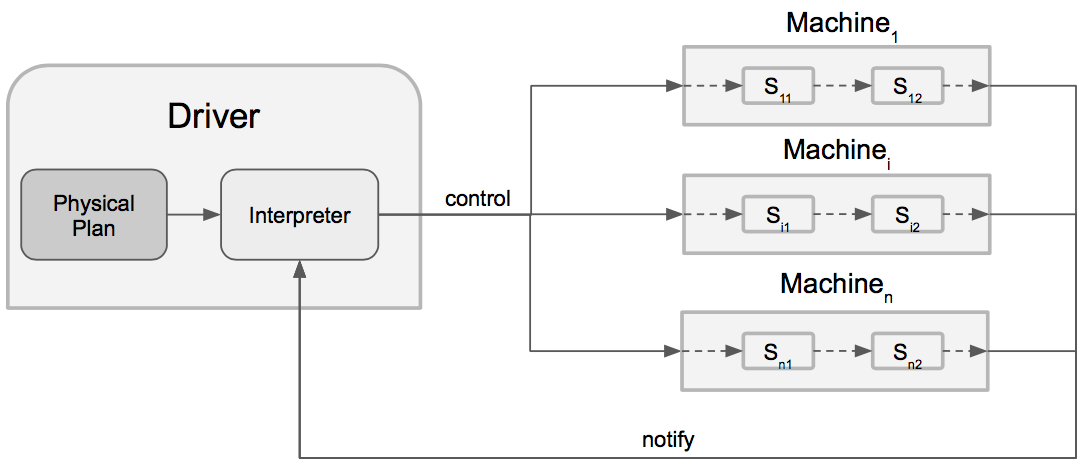
\includegraphics[width=0.8\textwidth]{img/framework_driver.png}
\caption{Algorithm Execution Architecture}
\label{fig:framework_driver}
\end{figure}
The machine running the interpreter is called the driver, which can be either a dedicated machine that is part of the cluster or the developers own machine.
According to the physical plan, a sequence of steps $S_{ij}, i \in \{1, \ldots, M\}, j \in \{1, 2\}$ is executed on each machine.
Each step can either be computation, or a control flow operator such as a loop, which in turn contains again a sequence of steps.


\section{State Centric Programming Model}
In order to support the development process, a programming model is required that is expressive enough to conveniently model the complex dependencies when executing a machine learning algorithm in a distributed manner.
For this purpose the framework provides a so called state centric programming model, which is motivated by means of the example algorithm definition in \ref{alg:general_ica}, describing a generic iterative-convergent algorithm as it would be implemented by a developer.
The algorithm definition is very similar among members of the ICA\footnote{iterative-convergent-algorithm} family, only $f_p$ and $\Delta(\ldots)$ must be replaced by the corresponding preprocessing transformation respectively the optimization technique used to iteratively approximating the optimal solution according to Section \ref{ss:optimization}.
\begin{algorithm}
\caption{Generic iterative-convergent algorithm}\label{alg:general_ica}
\begin{algorithmic}[1]{}
\ALGSTATE Data tensor $D \in \mathbb{R}^{n \times d}$, weight tensor $w \in \mathbb{R}^{m \times d}$
\INPUT algorithm specific hyper-parameters $\theta$, if any
\INIT $t \gets 0$, $w^{(0)} \gets 0$
\State $D \gets f_{p}(D)$ \Comment{(A)}
\Repeat \Comment{(B)}
\State $t \gets t + 1$
\State $w^{(t)} \gets w^{(t-1)} + \Delta(w^{(t-1)}, \theta, D)$ \Comment{(C)}
\Until{termination criteria satisfied} \Comment{(D)}
\end{algorithmic}
\end{algorithm}
Figure \ref{fig:ica_control_flow} depicts (\ref{alg:general_ica}) from a control-flow perspective, describing the algorithm in terms of a sequence of nested operators such as computation/transformation, loops and branches.
\begin{figure}[ht]
\centering
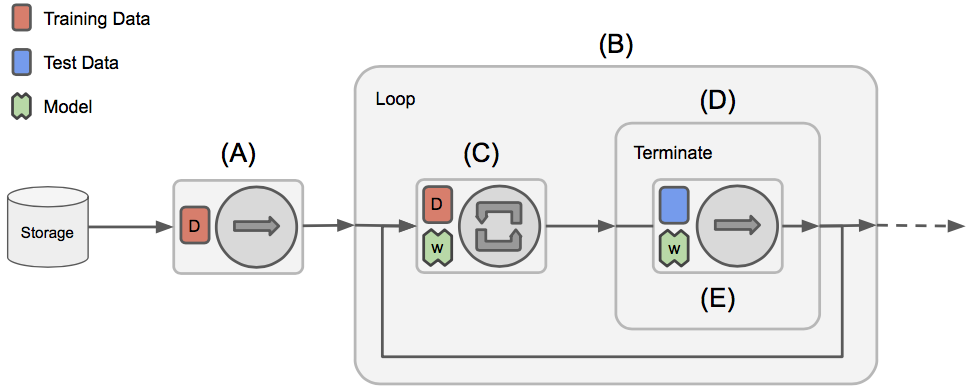
\includegraphics[width=0.9\textwidth]{img/ica_control_flow.png}
\caption{Iterative-convergent algorithm control-flow}
\label{fig:ica_control_flow}
\end{figure}
The algorithm starts with loading the input data $D$ from an arbitrary storage, followed by one ore more preprocessing steps (e.g. normalization or standardization as well as splitting the data into training and test set \textbf{(A)}).
A square represents a step of the algorithm, which contains an arbitrary number of input states (e.g. data, model) and some kind of transformation or computation applied to them.
This step is called a unit and is described in more detail in Section \ref{ss:unit}.
A transformation is depicted as a circle and can either be applied once (arrow) or multiple times (cyclic arrows) to the state(s) during this particular step.
After applying the preprocessing the actual training process is triggered, which is contained in a loop \textbf{(B)}.
A loop symbolizes that the containing steps are executed repeatedly until some termination criterion \textbf{(D)} is satisfied, which is computed in \textbf{(E)}.
For most machine learning algorithms the termination criterion can either be a fixed number of iterations, the change in objective $Q$ between iterations or the generalization performance.
\textbf{(C)} is the actual training step which iteratively refines the model by updates computed from the input data according to \ref{eqn:delta_upd}.
It can already be seen from the example that the framework must be capable of executing a complex sequence of arbitrary control flow operators and transformation steps in parallel on multiple machines.
The framework therefore defines primitives to define the control flow as well as units and state.
An algorithm expressed in this form could be executed as is on a single machine without modification because its sequential, non-parallel execution ensures the consistency of all involved states throughout the algorithm execution.
Consistency in this context means that, because of its sequential execution, no conflicts can occur when altering a particular state as described in Section \ref{ss:consistency}.
Distributing said algorithm therefore requires additional instructions on how to ensure that conflicts can be resolved properly.
These instructions are then combined with the logical representation of the algorithm and additional information regarding the distribution of state and the cluster environment to obtain a physical representation.
This is the responsibility of the algorithm parallelization pipeline, described in Section \ref{s:algo_parallel_pipeline}, which takes the algorithm definition as input and returns a physical plan.
The next sections introduce the key elements of the programming model.

\subsection{State}
Assuming the algorithm described in (\ref{alg:general_ica}) should be parallelized with a dop\footnote{degree of parallelism} of two, it is necessary to replicate each transformation step of the sequential algorithm on $K = 2$ machines, as shown in Figure \ref{fig:ica_control_flow_dist}.
\begin{figure}[ht]
\centering
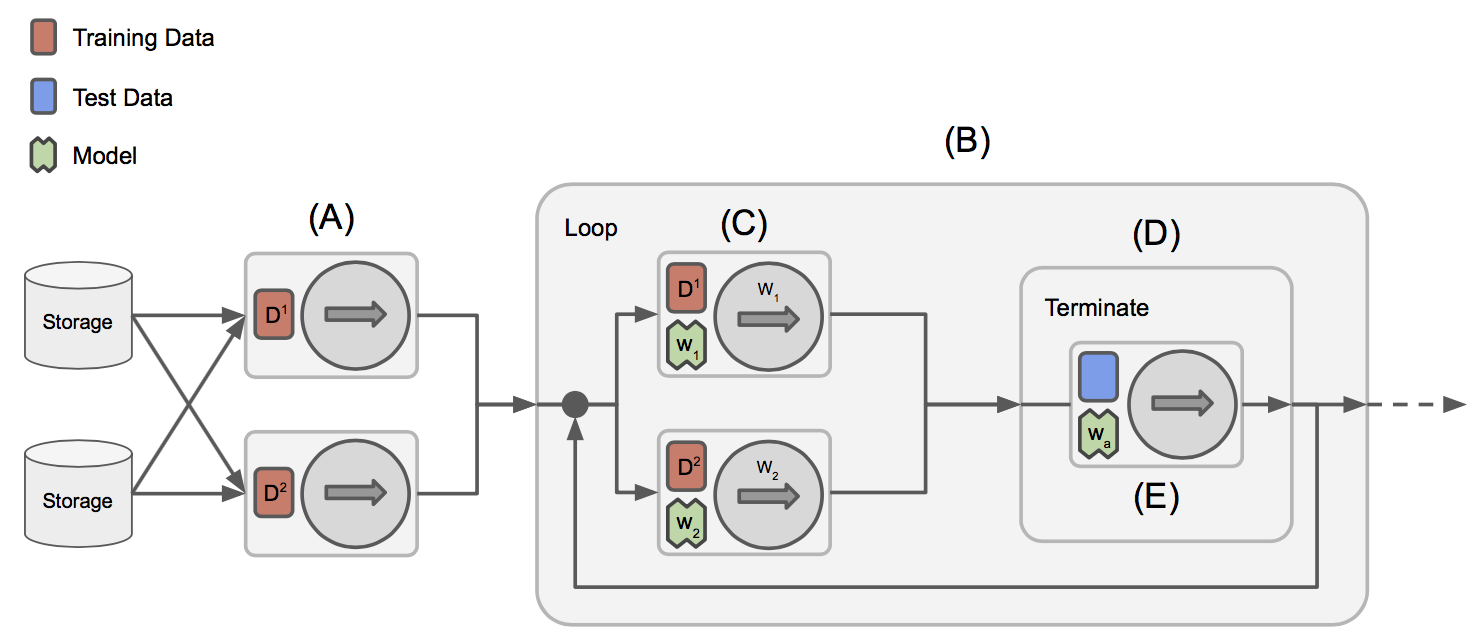
\includegraphics[width=0.9\textwidth]{img/ica_control_flow_dist.png}
\caption{Distributed Machine Learning Pipeline for Iterative-convergent Algorithms}
\label{fig:ica_control_flow_dist}
\end{figure}
It is worth noting that the transformation logic stays the same independently of the degree-of-parallelism, including a dop of one, which is essentially a single machine.
Therefore the framework instead of distributing the transformation focuses on how to distribute the state and keeping it consistent throughout the execution of each transformation step.
Hence the programming model introduces the concept of state, which is essentially a container for an arbitrary, distributable data structure.
A state $\gamma$ must be partitionable, meaning it can be distributed according to a partitioning $\{P_{\gamma}\}_{k=1}^K$, where $K$ is the degree of parallelism.
In the area of machine learning, state is commonly represented by tensors of arbitrary type, such as floating point numbers, integers or strings.
Therefore any further discussion assumes that a state is represented by a tensor of order two (matrix).
For example the algorithm in (\ref{alg:general_ica}) requires two states, namely the input data $D$ and the model $w$.
In order to parallelize the algorithm, the parallelization pipeline requires a partitioning $\{P_\gamma\}_{k=1}^K$ for both states, which in the context of machine learning can be divided into the following cases, shown in Table \ref{tab:ica_partitioning}.
\begin{table}[h]
\begin{center}
\begin{tabular}{ | c | c | c |}
\hline
$\gamma_w \setminus \gamma_D$ & partitioned & replicated \\ \hline
partitioned & $\gamma_w^S \wedge \gamma_D^T$ &  $\gamma_w^S \wedge \gamma_{D_T}$\\ \hline
replicated & $\gamma_{w_S} \wedge \gamma_D^T$ & $\times$\\
\hline
\end{tabular}
\label{tab:ica_partitioning}
\caption{Distributed Machine Learning Pipeline for Iterative-convergent Algorithms}
\end{center}
\end{table}
Where $S \subset \{1, \ldots, M\}$ and $T \subset \{1, \ldots, M\}$, with $M$ being the number of available machines in the cluster and $\mid S \mid = \mid T \mid = K$.
In this context, a subscript set of indices means the state is replicated among the set of machines, whereas a superscript set of indices indicates the state is partitioned among the set of machines.
As described in Section \ref{ss:state_partitioning}, $w_S \wedge D^T$ equals data-parallelism, $w^S \wedge D_T$ equals model-parallelism and $w^S \wedge D^T$ is a hybrid approach that is often used in a parameter server setup where model and input data are both distributed among a set of machines.
The example in Figure \ref{fig:ica_control_flow_dist} therefore depicts a data-parallel approach because the input data $D$ is partitioned into $D^{\{1,2\}}$, whereas the model $w$ is replicated across machines $w_{\{1,2\}}$.
In general the distribution of state in machine learning depends on the size of the problem and the algorithm employed to obtain an optimal solution for the given objective.
E.g. in cases where the model $w$ does not fit into the memory of a single machine it is partitioned among a sufficient number of machines.
The same holds for the size of the input data $D$.
A special case is the partitioning $\{P_D\}_{k=1}^K$ of the input data, which is in general a matrix with rows consisting of examples.
For iterative-convergent algorithms, depending on the optimization technique used to iteratively optimize the objective $Q$ of interest, two partitioning schemes are commonly used.
If the optimization technique requires access to a complete example in order to update the model, such as it is the case with stochastic gradient descent, the input data is partitioned row-wise.
On the other hand, if a coordinate-wise optimization technique is used which only needs access to a single feature, the input data is distributed column-wise as shown in Figure \ref{fig:row_col_dist} for a dop of two.
\begin{figure}[ht]
\centering
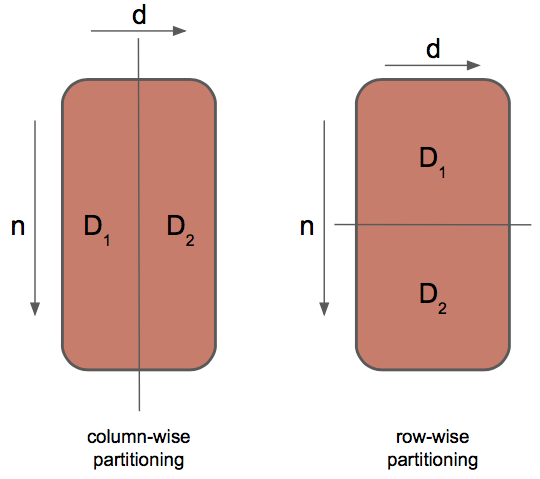
\includegraphics[width=0.4\textwidth]{img/row_col_dist.png}
\caption{Partitioning of input data in distributed machine learning}
\label{fig:row_col_dist}
\end{figure}

\subsection{Unit}
\label{ss:unit}
As shown in Figure \ref{fig:ica_control_flow_dist}, distributing the algorithm not only requires the state to be distributed but also the transformation applied to the state must be replicated and executed in parallel across a set of machines.
For this purpose the framework provides a primitive to define a unit of work.
A unit $\Omega$ can be thought of as a function, taking an arbitrary number of states as input and either transforming the input state(s) or updating a state based on an update computed from the input.
More specifically a unit defines an atomic step of an algorithm, described by the state centric programming model.
This is necessary because each unit spans a scope for the consistency management and further instructions may be provided in order to ensure a consistent, efficient, distributed execution of the work defined in this particular unit.
For this to work, the transformation or computation defined in a unit must satisfy an independence property regarding the input states, meaning that the work can be applied to a partition of the input state(s) without changes.
Figure \ref{fig:unit} depicts the general layout of a unit.
\begin{figure}[ht]
\centering
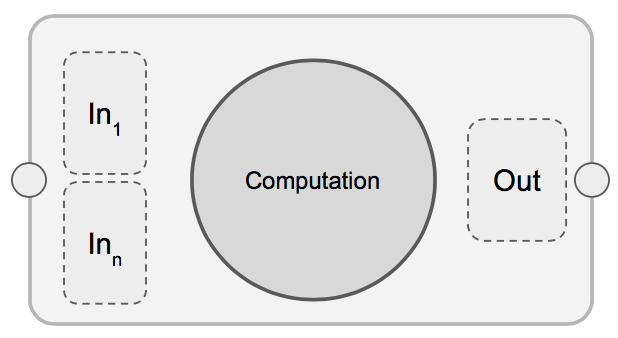
\includegraphics[width=0.4\textwidth]{img/unit.png}
\caption{Layout of a Unit}
\label{fig:unit}
\end{figure}
The connectors describe an interface for receiving a control flow signal, triggering the execution of the unit and emitting a control flow signal after the work is done.
This is used by the interpreter to schedule and execute units according to the control-flow described in the physical plan compiled by the algorithm parallelization pipeline.
Figure \ref{fig:driver_units} shows two units chained together, where the first unit triggers the execution of the second unit, which in turn notifies the interpreter after the work is done.
This closely resembles the control flow known from imperative programming languages, the difference is that this control flow can be distributed with an arbitrary degree of parallelism on a set of machines in a cluster.
\begin{figure}[ht]
\centering
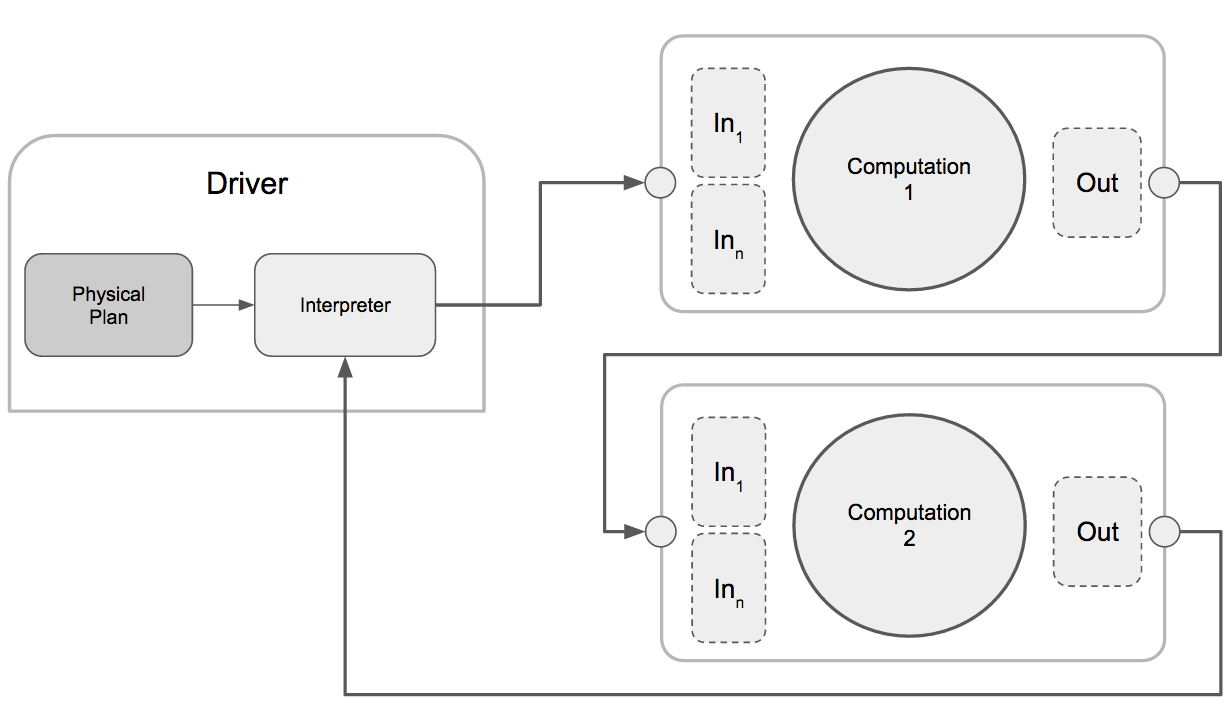
\includegraphics[width=0.8\textwidth]{img/driver_units.png}
\caption{Units controlled by the Driver}
\label{fig:driver_units}
\end{figure}

\subsection{Synchronization}
As mentioned before, when distributing an algorithm, each unit scope has different requirements regarding consistency.
As shown in Figure \ref{fig:ica_control_flow_dist}, the input state $D$ is partitioned into $K = 2$ parts, which means that also the units must be replicated $K$ times.
First, in order to ensure a correct parallel execution, the consistency management must ensure that all parallel instances of a unit are properly synchronized according to the schemes discussed in Section \ref{ss:consistency}.
This synchronization happens on the control flow level and instructions on how to synchronize a unit or a control-flow operator such as a loop must be provided by the developer.
In case of the example, the preprocessing step (A) must be finished before the next step (B) can be triggered.
Therefore the parallel instances of unit (A) must be BSP, which is the default in case no further instructions are provided for unit synchronization.
Things are different for step (B), which is the loop containing the training step.
In order to improve performance, this loop is often executed with SSP or TAP synchronization, meaning that the parallel instances of unit (C) can be executed in parallel without the need to synchronize on the outer loop.
This increases the data throughput and therefore the overall performance.
Secondly, as the parallel instances of a unit span a consistency scope, as can be seen in Figure \ref{fig:consistency_scope}, consistency management must also ensure consistency on a state level, which is discussed in the next chapter.
\begin{figure}[ht]
\centering
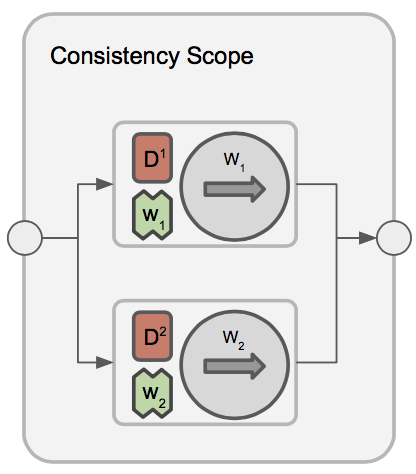
\includegraphics[width=0.3\textwidth]{img/consistency_scope.png}
\caption{Consistency Scope of parallel Units}
\label{fig:consistency_scope}
\end{figure}

\subsection{Framework in Action}
This section combines the primitives introduced in the previous sections with the example machine learning algorithm definition in (\ref{alg:general_ica}) in order to show how it can be utilized by a developer to distribute said algorithm.
In addition to the original definition, a partitioning is required for each of the states $D$ and $w$ serving as instructions for the framework on how to distribute the state.
Furthermore the unit scopes $\Omega_1, \Omega_2$ must be defined within the algorithm and additionally the synchronization scheme must be specified in order for the consistency management to work properly.
\begin{algorithm}
\caption{SCPM iterative-convergent algorithm definition}\label{alg:scpm_ica}
\begin{algorithmic}[1]{}
\ALGSTATE Data tensor $D \in \mathbb{R}^{n \times d}$, weight tensor $w \in \mathbb{R}^{m \times d}$
\PARTITIONING $\{P_D\}_{k=1}^K$, $\{P_w\}_{k=1}^K$
\INPUT algorithm specific hyper-parameters $\theta$, if any
\INIT $t \gets 0$, $w^{(0)} \gets 0$
\State \textbf{with} \textit{BSP}
\State \hspace{\algorithmicindent} $\Omega_1[D \gets f_{p}(D)]$
\Repeat
\State \textbf{with} \textit{SSP}
\State \hspace{\algorithmicindent} $\Omega_2[t \gets t + 1]$
\State \hspace{\algorithmicindent} $\Omega_2[w^{(t)} \gets w^{(t-1)} + \Delta(w^{(t-1)}, \theta, D)]$
\Until{termination criteria satisfied}
\end{algorithmic}
\end{algorithm}


\section{Algorithm Parallelization Pipeline}
\label{s:algo_parallel_pipeline}
The algorithm parallelization pipeline is part of the framework and provides the functionality to translate an algorithm defined with the state centric programming model (\ref{alg:scpm_ica}) into a representation suited for distributed execution by the driver.
The sequence of steps to go from an algorithm definition to a distributed or physical plan is depicted in Figure \ref{fig:parallel_pipeline}, where a dark arrow resembles an intermediate representation and a light arrow depicts a transformation step between those representations.
At first, a logical plan is derived from the algorithm definition by the compiler, which is then passed on to the parallelizer.
The logical plan is then combined with information about the cluster, such as the available resources on each machine and further instructions for the consistency management, to obtain a physical plan that is used by the driver to actually schedule the distributed execution of the algorithm in the cluster.
\begin{figure}[ht]
\centering
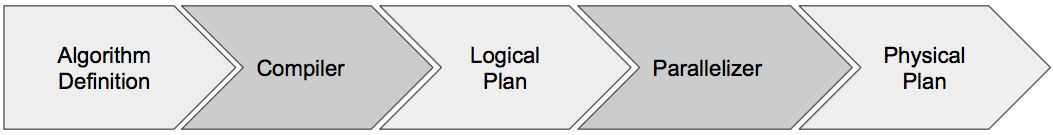
\includegraphics[width=0.9\textwidth]{img/algo_parallel_pipeline.png}
\caption{Algorithm parallelization pipeline}
\label{fig:parallel_pipeline}
\end{figure}
The following sections describe each step and the resulting intermediate representation in more detail.

\subsection{Compiler}
The compiler is the first step in the algorithm parallelization pipeline and it is responsible for building a logical representation of the algorithm, or logical plan by analyzing the algorithm definition.
Figure \ref{fig:logical_plan} shows the logical plan derived from the example definition in (\ref{alg:scpm_ica}).
\begin{figure}[ht]
\centering
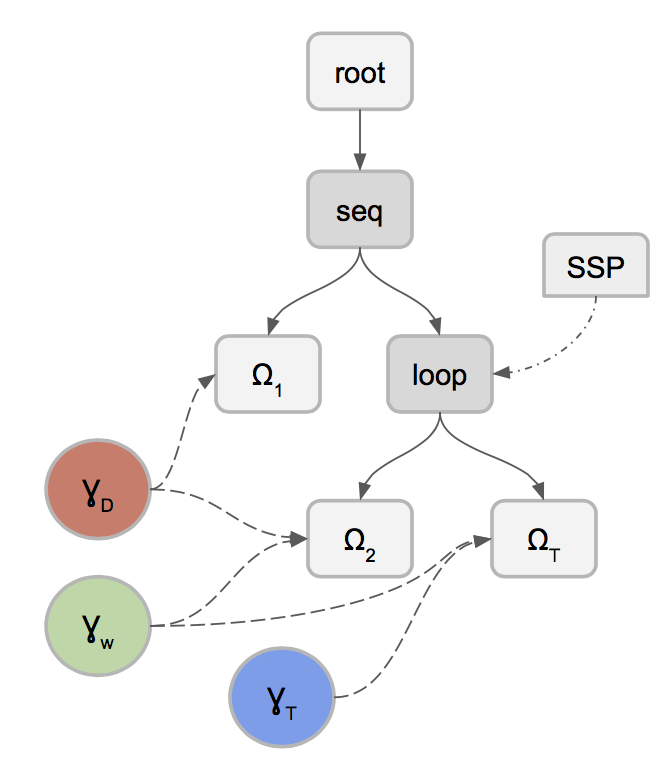
\includegraphics[width=0.4\textwidth]{img/logical_plan.png}
\caption{Logical Plan}
\label{fig:logical_plan}
\end{figure}
At first a tree is built, resembling the control-flow of the algorithm, with intermediate nodes describing a control-flow operator (sequential, parallel, loop) and the leafs consist of units $\Omega_{ij}$ with $i \in \{1, \ldots, M\}$ and $j \in \{1, \ldots, U\}$, where $U$ is the number of distinct units.
Leafs always consist of units as these are the atomic parts of an algorithm and therefore can not be further divided.
The next step connects all states $\gamma$ with the units $\Omega$ that need access to a particular state.
This is then used to identify when a specific state must be created and when it can be safely disposed.
For example $\gamma_D$ is required in unit $\Omega_1$ and $\Omega_2$, which is denoted by $\Omega(\gamma_D) = \{1, 2\}$.
Finally the synchronization instructions for the consistency management are attached to the units and control-flow operators according to the definition.
In case of the example, the loop operator should be executed using SSP.
Control-flow operators and unit without additional synchronization instructions default to BSP.
It is worth noting that the logical plan is built using only the information derived from the algorithm definition.
One can think of the logical plan as an abstract representation of the algorithm, which can be parallelized in different ways by providing further instructions such as the degree of parallelism or the architecture of the cluster.
This information is then used by the parallelizer to built a specific architecture dependent physical plan.

\subsection{Parallelizer}
The second step in the parallelization pipeline is the parallelizer.
It receives the logical plan of the compiler and combines it with additional information required to derive an executable, physical plan from it.
Figure \ref{fig:physical_plan} shows the physical plan corresponding to the logical plan in Figure \ref{fig:logical_plan}.
\begin{figure}[ht]
\centering
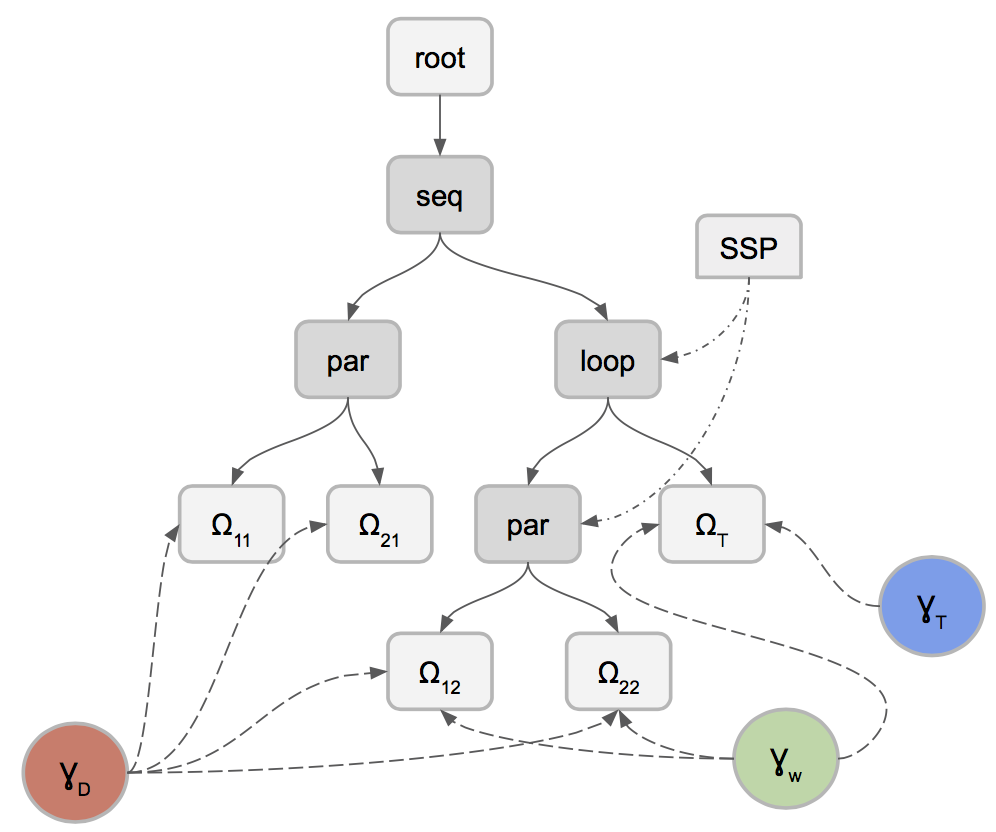
\includegraphics[width=0.7\textwidth]{img/physical_plan.png}
\caption{Physical Plan}
\label{fig:physical_plan}
\end{figure}
As in the previous example, a dop of two is used and the parallelizer transforms the logical plan into a physical plan with distributed control-flow for the interpreter.
The parallelizer first uses the dop $k$ to distribute each state according to the configured partitioning $\{P_{\gamma}\}_{k=1}^K$, which also implies that the corresponding units must be replicated $k$ times.
Each unit $\Omega_j$ is translated into a parallel control-flow operator containing the replicas $\Omega_{ij}$ for $i \in \{1, \ldots, k\}$.
Furthermore a machine is assigned to each unit so it can be scheduled accordingly by the interpreter.
The parallelizer also must take care of the locality of state and schedule the units accordingly.

\textbf{NOTES:} termination criterion should be something like until $f_T(w, D_{test})$ equals true, this enables the use of $\Omega_T$ as unit
